% === T07 - Arquitectura de procesadores ===
% David Alejandro Gonzalez Marquez
% fokerman@gmail.com
% https://github.com/fokerman/computingSystemsCourse

\documentclass[aspectratio=169]{beamer}
% \documentclass[aspectratio=169, handout]{beamer}

% % % Packages
\usepackage[sfdefault]{AlegreyaSans}
\usepackage{inconsolata}
\usepackage{multicol}
\usepackage{multirow}
\usepackage[spanish]{babel}
\usepackage[utf8]{inputenc}
\usepackage{enumerate}
\usepackage{color}
\usepackage{xcolor}
\usepackage[absolute,overlay]{textpos}
  \setlength{\TPHorizModule}{1mm}
  \setlength{\TPVertModule}{1mm}
\usepackage{framed}
\usepackage{mfirstuc} % para poner en mayusculas la primer letra
\usepackage{xspace} % para crear espacios en comandos 
\usepackage{pbox}
\usepackage{tikz}
\usepackage{mathabx}
\usepackage{colortbl}
\usepackage{ulem} % para tener tachado

% % % Beamer config
\usetheme{Pittsburgh}
\usecolortheme[rgb={1,0.48,0.0}]{structure}
\setbeamercolor{block title}{fg=white,bg=verdeuca}
\xdefinecolor{verdeuca}{rgb}{0.0,0.48,0.54}
\xdefinecolor{naranjauca}{rgb}{1,0.48,0.0}
\setbeamercolor{palette quaternary}{fg=white,bg=verdeuca}
\setbeamertemplate{title page}[default][colsep=-4bp, rounded=true] % remove title shadow
\setbeamertemplate{frametitle}[default][colsep=-2bp, shadow=false] % remove frame title shadow
\setbeamertemplate{navigation symbols}{} % remove navigation symbols
\beamertemplatenavigationsymbolsempty

% % % Colors
\definecolor{Gris}{gray}{0.8}
\definecolor{Celeste}{rgb}{.255,.41,.884}
\definecolor{Rojo}{rgb}{1, 0, 0}
\definecolor{a}{rgb}{0.0, 0.53, 0.74}
\definecolor{r}{rgb}{0.89, 0.0, 0.13}
\definecolor{v}{rgb}{0.0, 0.5, 0.0}
\definecolor{y}{rgb}{0.0, 0.5, 0.5}
\definecolor{rojo}{HTML}{F1521B}
\definecolor{verde}{HTML}{80CD29}
\definecolor{amarillo}{HTML}{FABC09}
\definecolor{azulC}{rgb}{.31,.506,.741}
\definecolor{azul}{HTML}{00ADF1}
\definecolor{verdeC}{HTML}{8FF0A4}
\definecolor{verdeO}{HTML}{2EC27E}

% % % Rename
\newcommand{\tab}[0]{\hspace{15pt}}

% % % Blocks
\setbeamercolor{block body}{fg=black, bg=black!10}
\setbeamercolor{block title}{fg=black, bg=black!20}
\setbeamercolor{coloredboxstuffNaranja}{fg=naranjauca,bg=black!10} %% PARA LOS BOX
\setbeamercolor{coloredboxstuffVerde}{fg=verdeuca,bg=black!10} %% PARA LOS BOX

% % % Special Packages
\usepackage{fontawesome}
\usepackage{pgf}

\usepackage{array}
\newcommand{\PreserveBackslash}[1]{\let\temp=\\#1\let\\=\temp}
\newcolumntype{C}[1]{>{\PreserveBackslash\centering}p{#1}}
\newcolumntype{R}[1]{>{\PreserveBackslash\raggedleft}p{#1}}
\newcolumntype{L}[1]{>{\PreserveBackslash\raggedright}p{#1}}

% % % Start
\title{\Huge Arquitectura de procesadores}
% \subtitle{}

\author{David Alejandro González Márquez}
\institute{}

\date{}

\begin{document}

\begin{frame}[plain]
    \titlepage
    \begin{textblock}{140}(10,70)
    \textcolor{rojo}{
    \textbf{Atención}: La clase será grabada por el anfitrión para su posterior y eventual uso académico dentro de nuestra institución. Su participación en la clase implica brindar su consentimiento para participar en la grabación, aunque pueden mantener su video apagado.}
    \end{textblock}
\end{frame}

\begin{frame}[fragile,t]{Arquitectura OrgaSmall}
    \small
    Para ilustrar el funcionamiento de un sistema de computo, vamos a presentar la arquitectura \emph{OrgaSmall}.\\
    \vspace{0.2cm}
    Esta arquitectura fue diseñada con fines didácticos y su objetivo es poner de manifiesto todos los conceptos básicos de la organización de un procesador con una arquitectura simple.\\
    \bigskip    
    \begin{textblock}{100}(10,30)
    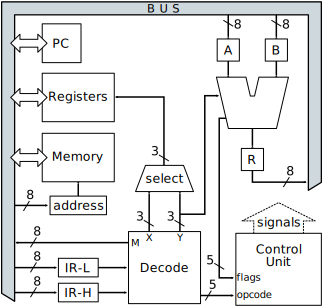
\includegraphics[scale=0.6]{img/arquitectura_micro.pdf}
    \end{textblock}
    \begin{textblock}{100}(70,30)
    \begin{itemize}
    \item 8 registros de propósito general, \texttt{R0} a \texttt{R7}.
    \item 1 registro de propósito específico PC.
    \item Unidad direccionable de 8 bits (1 byte) e \\ instrucciones de 16 bits (2 bytes).
    \item Memoria de 256 bytes.
    \item Bus de 8 bits.
    \item Diseño microprogramado.
    \end{itemize}
    \end{textblock}
\end{frame}

\begin{frame}[fragile,t]{Arquitectura OrgaSmall}{Conjunto de instrucciones}
    \begin{textblock}{55}(5,19)
    \small
    \textbf{Decodificación}\\
    \scriptsize
    Instrucciones de 16 bits.
    Los primeros 5 bits identifican el \texttt{opcode} de la instrucción, el resto de los bits indican los parámetros.\\
    \bigskip
    \textbf{\texttt{Rx} o \texttt{Ry}}: Índices de registros, número entre \texttt{0} y \texttt{7}.\\
    \textbf{\texttt{M}}: Dirección de memoria o valor inmediato, número de 8 bits.\\
    \textbf{\texttt{t}}: Valor inmediato de desplazamiento, número entre \texttt{0} y \texttt{7}. Se codifica como \texttt{YYY} en 3 bits.\\
    \bigskip
    \uncover<2->{\small \textcolor{gray}{Ejemplos}\\}
    \vspace{0.2cm}
    \footnotesize
    \begin{tabular}{l|c}
    \uncover<2->{ Instrucción             & Codificación \\ \hline }
    \uncover<2->{ \texttt{ADD R3, R6}     & }\uncover<3->{\texttt{\textcolor{r}{00001}\textcolor{v}{011}\textcolor{verde}{110}\textcolor{gray}{00000}} } \\  %01
    \uncover<2->{ \texttt{STR [0x21], R5} & }\uncover<4->{\texttt{\textcolor{r}{10000}\textcolor{v}{101}\textcolor{a}{00100001}} } \\  %16
    \uncover<2->{ \texttt{SET R1, 0xFF}   & }\uncover<5->{\texttt{\textcolor{r}{11111}\textcolor{v}{001}\textcolor{a}{11111111}} } \\  %31
    \uncover<2->{ \texttt{SHL R7, 3}      & }\uncover<6->{\texttt{\textcolor{r}{11011}\textcolor{v}{111}\textcolor{verde}{011}\textcolor{gray}{00000}} } \\  %27
    \end{tabular}
    \end{textblock}
    \begin{textblock}{100}(65,8)
    \scriptsize
    \begin{tabular}{l|l|l}
    Instrucción            & Acción                                                             & Codificación               \\
    \hline
    \texttt{ADD  Rx, Ry}   & \texttt{Rx} $\leftarrow$ \texttt{Rx + Ry}                          & \texttt{\textcolor{r}{00001}\textcolor{v}{XXX}\textcolor{verde}{YYY}\textcolor{gray}{-----}} \\  %01
    \texttt{ADC  Rx, Ry}   & \texttt{Rx} $\leftarrow$ \texttt{Rx + Ry + flag\_C}                & \texttt{\textcolor{r}{00010}\textcolor{v}{XXX}\textcolor{verde}{YYY}\textcolor{gray}{-----}} \\  %02
    \texttt{SUB  Rx, Ry}   & \texttt{Rx} $\leftarrow$ \texttt{Rx - Ry}                          & \texttt{\textcolor{r}{00011}\textcolor{v}{XXX}\textcolor{verde}{YYY}\textcolor{gray}{-----}} \\  %03
    \texttt{AND  Rx, Ry}   & \texttt{Rx} $\leftarrow$ \texttt{Rx and Ry}                        & \texttt{\textcolor{r}{00100}\textcolor{v}{XXX}\textcolor{verde}{YYY}\textcolor{gray}{-----}} \\  %04
    \texttt{OR   Rx, Ry}   & \texttt{Rx} $\leftarrow$ \texttt{Rx or Ry}                         & \texttt{\textcolor{r}{00101}\textcolor{v}{XXX}\textcolor{verde}{YYY}\textcolor{gray}{-----}} \\  %05
    \texttt{XOR  Rx, Ry}   & \texttt{Rx} $\leftarrow$ \texttt{Rx xor Ry}                        & \texttt{\textcolor{r}{00110}\textcolor{v}{XXX}\textcolor{verde}{YYY}\textcolor{gray}{-----}} \\  %06
    \texttt{CMP  Rx, Ry}   & Modifica \emph{flags} de \texttt{Rx - Ry}                          & \texttt{\textcolor{r}{00111}\textcolor{v}{XXX}\textcolor{verde}{YYY}\textcolor{gray}{-----}} \\  %07
    \texttt{MOV  Rx, Ry}   & \texttt{Rx} $\leftarrow$ \texttt{Ry}                               & \texttt{\textcolor{r}{01000}\textcolor{v}{XXX}\textcolor{verde}{YYY}\textcolor{gray}{-----}} \\  %08
    \hline
    \texttt{STR  [M], Rx}  & \texttt{Mem[M]} $\leftarrow$ \texttt{Rx}                           & \texttt{\textcolor{r}{10000}\textcolor{v}{XXX}\textcolor{a}{MMMMMMMM}} \\  %16
    \texttt{LOAD Rx, [M]}  & \texttt{Rx} $\leftarrow$ \texttt{Mem[M]}                           & \texttt{\textcolor{r}{10001}\textcolor{v}{XXX}\textcolor{a}{MMMMMMMM}} \\  %17
    \texttt{STR  [Rx], Ry} & \texttt{Mem[Rx]} $\leftarrow$ \texttt{Ry}                          & \texttt{\textcolor{r}{10010}\textcolor{v}{XXX}\textcolor{verde}{YYY}\textcolor{gray}{-----}} \\  %18
    \texttt{LOAD Rx, [Ry]} & \texttt{Rx} $\leftarrow$ \texttt{Mem[Ry]}                          & \texttt{\textcolor{r}{10011}\textcolor{v}{XXX}\textcolor{verde}{YYY}\textcolor{gray}{-----}} \\  %19
    \hline
    \texttt{JMP M}         & \texttt{PC} $\leftarrow$ \texttt{M}                                & \texttt{\textcolor{r}{10100}\textcolor{gray}{---}\textcolor{a}{MMMMMMMM}} \\  %20
    \texttt{JC M}          & Si \texttt{flag\_C=1} entonces \texttt{PC} $\leftarrow$ \texttt{M} & \texttt{\textcolor{r}{10101}\textcolor{gray}{---}\textcolor{a}{MMMMMMMM}} \\  %21
    \texttt{JZ M}          & Si \texttt{flag\_Z=1} entonces \texttt{PC} $\leftarrow$ \texttt{M} & \texttt{\textcolor{r}{10110}\textcolor{gray}{---}\textcolor{a}{MMMMMMMM}} \\  %22
    \texttt{JN M}          & Si \texttt{flag\_N=1} entonces \texttt{PC} $\leftarrow$ \texttt{M} & \texttt{\textcolor{r}{10111}\textcolor{gray}{---}\textcolor{a}{MMMMMMMM}} \\  %23
    \hline
    \texttt{INC Rx}        & \texttt{Rx} $\leftarrow$ \texttt{Rx + 1}                           & \texttt{\textcolor{r}{11000}\textcolor{v}{XXX}\textcolor{gray}{--------}} \\  %24
    \texttt{DEC Rx}        & \texttt{Rx} $\leftarrow$ \texttt{Rx - 1}                           & \texttt{\textcolor{r}{11001}\textcolor{v}{XXX}\textcolor{gray}{--------}} \\  %25
    \texttt{SHR Rx, t}     & \texttt{Rx} $\leftarrow$ \texttt{Rx} \verb|<<| \texttt{t}          & \texttt{\textcolor{r}{11010}\textcolor{v}{XXX}\textcolor{verde}{YYY}\textcolor{gray}{-----}} \\  %26
    \texttt{SHL Rx, t}     & \texttt{Rx} $\leftarrow$ \texttt{Rx} \verb|>>| \texttt{t}          & \texttt{\textcolor{r}{11011}\textcolor{v}{XXX}\textcolor{verde}{YYY}\textcolor{gray}{-----}} \\  %27
    \hline
    \texttt{SET Rx, M}     & \texttt{Rx} $\leftarrow$ \texttt{M}                                & \texttt{\textcolor{r}{11111}\textcolor{v}{XXX}\textcolor{a}{MMMMMMMM}} \\  %31
    \end{tabular}\\
    \vspace{0.2cm}
    Los bits indicados con \textcolor{gray}{\texttt{-}} deben valer cero.
    \end{textblock}
\end{frame}

\begin{frame}[fragile,t]{Arquitectura OrgaSmall}{Ejemplos en lenguaje ensamblador}
    \begin{textblock}{60}(10,13)
    \begin{center}
    Ejemplo Sumas
    \end{center}
    \end{textblock}
    \begin{textblock}{100}(10,23)
    \textcolor{naranjauca}{Ensamblador}
    \begin{verbatim}
      SET R0, 0x01
      SET R1, 0x05
next: ADD R0, R1
      JMP next
    \end{verbatim}
    \end{textblock}
    \begin{textblock}{100}(50,23)
    \color{gray}
    Memoria
    \begin{verbatim}
00 | f8 01 
02 | f9 05 
04 | 08 20 
06 | a0 04
    \end{verbatim}
    \color{black}
    \end{textblock}
    \begin{textblock}{100}(80,5)
    \textbf{Seguimiento}\\
    \small \textcolor{verdeuca}{Suponer inicialmente todos los registros en cero.}
    \normalsize
    \begin{tabular}{|c|l|l|} \hline
    \texttt{PC} & Instrucción            & Resultado \\ \hline
    \uncover<2->{\texttt{00} } & \uncover<2->{\texttt{SET R0, 0x01} } & \uncover<2->{\texttt{R0 $\leftarrow$ 01} } \\
    \uncover<3->{\texttt{02} } & \uncover<3->{\texttt{SET R1, 0x05} } & \uncover<3->{\texttt{R1 $\leftarrow$ 05} } \\
    \uncover<4->{\texttt{04} } & \uncover<4->{\texttt{ADD R0, R1}   } & \uncover<4->{\texttt{R0 $\leftarrow$ 05+01 = 06} } \\
    \uncover<5->{\texttt{06} } & \uncover<5->{\texttt{JMP next}     } & \uncover<5->{\texttt{PC $\leftarrow$ 04} } \\
    \uncover<6->{\texttt{04} } & \uncover<6->{\texttt{ADD R0, R1}   } & \uncover<6->{\texttt{R0 $\leftarrow$ 06+05 = 0B} } \\
    \uncover<7->{\texttt{06} } & \uncover<7->{\texttt{JMP next}     } & \uncover<7->{\texttt{PC $\leftarrow$ 04} } \\
    \uncover<7->{\texttt{04} } & \uncover<7->{\texttt{ADD R0, R1}   } & \uncover<7->{\texttt{R0 $\leftarrow$ 0B+05 = 10} } \\
    \uncover<7->{\texttt{06} } & \uncover<7->{\texttt{JMP next}     } & \uncover<7->{\texttt{PC $\leftarrow$ 04} } \\
    \uncover<7->{\texttt{04} } & \uncover<7->{\texttt{ADD R0, R1}   } & \uncover<7->{\texttt{R0 $\leftarrow$ 10+05 = 15} } \\
    \uncover<7->{\texttt{06} } & \uncover<7->{\texttt{JMP next}     } & \uncover<7->{\texttt{PC $\leftarrow$ 04} } \\
    \uncover<7->{\texttt{04} } & \uncover<7->{\texttt{ADD R0, R1}   } & \uncover<7->{\texttt{R0 $\leftarrow$ 15+05 = 1A}} \\ 
    \uncover<7->{$\cdots$    } & \uncover<7->{$\cdots$              } & \uncover<7->{$\cdots$} \\ 
    \end{tabular}
    \end{textblock}
    \begin{textblock}{45}(20,60)
    \only<5->{
    \scriptsize
    \textcolor{verdeuca}{
    \textbf{Nota:}\\
    \texttt{next} es una etiqueta, en ASM escribimos nombres que el ensablador convierte en direcciones de memoria.}\\
    \texttt{next} corresponde a la dirección de memoria \texttt{0x04}.
    }
    \end{textblock}
\end{frame}

\begin{frame}[fragile,t]{Arquitectura OrgaSmall}{Ejemplos en lenguaje ensamblador}
    \begin{textblock}{60}(10,13)
    \begin{center}
    Ejemplo Mayor de 3
    \end{center}
    \end{textblock}
    \begin{textblock}{100}(10,23)
    \scriptsize
    \textcolor{naranjauca}{Ensamblador}
    \vspace{-0.3cm}
    \begin{verbatim}
max3:   LOAD R1, [data1]
        LOAD R2, [data2]
        LOAD R3, [data3]
        CMP R1, R2
        JN maxR2
        MOV R0, R1
        JMP nextR3
maxR2:  MOV R0, R2
nextR3: CMP R0, R3
        JN maxR3
        JMP fin
maxR3:  MOV R0, R3
fin:    STR [mayor], R0
halt:   JMP halt
data1:  DB 0x35
data2:  DB 0x64
data3:  DB 0x33
mayor:  DB 0x00
    \end{verbatim}
    \end{textblock}
    \begin{textblock}{100}(50,23)
    \scriptsize
    \color{gray}
    Memoria
    \vspace{-0.3cm}
    \begin{verbatim}
00 | 89 1c
02 | 8a 1d
04 | 8b 1e
06 | 39 40
08 | b8 0e
0a | 40 20
0c | a0 10
0e | 40 40
10 | 38 60
12 | b8 16
14 | a0 18
16 | 40 60
18 | 80 1f
1a | a0 1a
1c | 35
1d | 64 
1e | 33 
1f | 00 
    \end{verbatim}
    \color{black}
    \end{textblock}
    \begin{textblock}{100}(80,5)
    \textbf{Seguimiento}\\
    \small \textcolor{verdeuca}{Suponer inicialmente todos los registros en cero.}
    \normalsize
    \begin{tabular}{|c|l|l|} \hline
    \texttt{PC} & Instrucción            & Resultado \\ \hline
    \uncover<2->{\texttt{00}  } & \uncover<2->{\texttt{LOAD R1, [data1]}  } & \uncover<2->{\texttt{R1 $\leftarrow$ 35}       } \\
    \uncover<3->{\texttt{02}  } & \uncover<3->{\texttt{LOAD R2, [data2]}  } & \uncover<3->{\texttt{R2 $\leftarrow$ 64}       } \\
    \uncover<4->{\texttt{04}  } & \uncover<4->{\texttt{LOAD R3, [data3]}  } & \uncover<4->{\texttt{R3 $\leftarrow$ 33}       } \\
    \uncover<5->{\texttt{06}  } & \uncover<5->{\texttt{CMP R1, R2}        } & \uncover<5->{\texttt{N $\leftarrow$ 1}         } \\
    \uncover<6->{\texttt{08}  } & \uncover<6->{\texttt{JN maxR2}          } & \uncover<6->{\texttt{PC $\leftarrow$ 0E}       } \\
    \uncover<7->{\texttt{0e}  } & \uncover<7->{\texttt{MOV R0, R2}        } & \uncover<7->{\texttt{R0 $\leftarrow$ 64}       } \\
    \uncover<8->{\texttt{10}  } & \uncover<8->{\texttt{CMP R0, R3}        } & \uncover<8->{\texttt{N $\leftarrow$ 0}         } \\
    \uncover<9->{\texttt{12}  } & \uncover<9->{\texttt{JN maxR3}          } & \uncover<9->{\texttt{PC $\leftarrow$ 14}       } \\
    \uncover<10->{\texttt{14} } & \uncover<10->{\texttt{JMP fin}          } & \uncover<10->{\texttt{PC $\leftarrow$ 18}      } \\
    \uncover<11->{\texttt{18} } & \uncover<11->{\texttt{STR [mayor], R0}  } & \uncover<11->{\texttt{MEM[1F] $\leftarrow$ 64} } \\
    \uncover<12->{\texttt{1a} } & \uncover<12->{\texttt{JMP halt}         } & \uncover<12->{\texttt{PC $\leftarrow$ 1A}      } \\ 
    \uncover<12->{$\cdots$    } & \uncover<12->{$\cdots$                  } & \uncover<12->{$\cdots$} \\
    \end{tabular}
    \end{textblock}
    \begin{textblock}{45}(80,78)
    \only<1->{
    \scriptsize
    \textcolor{verdeuca}{
    \textbf{Nota:}\\
    \texttt{DB} (Define Byte) es una meta instrucción que permite escribir bytes en la memoria.}
    } 
    \end{textblock}
\end{frame}

\begin{frame}[fragile,t]{Arquitecturas}
    \begin{textblock}{65}(80,10)
    \begin{center}
    Arquitectura Harvard\\
    \vspace{0.2cm}
    \includegraphics[scale=0.5]{img/arquitectura-layer1.pdf}
    \end{center}
    \begin{itemize}
    \scriptsize
    \item Tienen \textbf{dos buses} para transferir simultáneamente datos e instrucciones desde \textbf{dos memorias independientes}.
    \item Las computadoras modernas utilizan una \textbf{versión modificada} teniendo buses separados para datos e instrucciones pero almacenamiento en una sola memoria.
    \item Las arquitecturas Harvard puras solo se utilizan en \textbf{microcontroladores} o sistemas integrados.
    \end{itemize}
    \end{textblock}
    \begin{textblock}{65}(10,10)
    \begin{center}
    Arquitectura Von Neumann\\
    \vspace{0.2cm}
    \includegraphics[scale=0.5]{img/arquitectura-layer2.pdf} 
    \end{center}
    \begin{itemize}
    \scriptsize
    \item Consiste en tres sistemas de hardware: una \textbf{unidad central de procesamiento} CPU con una unidad de control, una ALU y registros. Una \textbf{memoria principal} que contiene datos y programas. Un subsistema de \textbf{entrada/salida}.
    \item Tiene la capacidad de ejecutar secuencialmente instrucciones. Contiene un único camino lógico entre la memoria principal y la unidad de control, forzando el acceso alternado entre datos e instrucciones. Este único camino es conocido como el \textbf{cuello de botella de von Neumann}.
    \end{itemize}
    \end{textblock}
\end{frame}

% \begin{frame}[fragile,t]{Arquitecturas}
% - Maquina de Pila
% - Maquina de Acumulador
% - Maquina de Registros
% \end{frame}

\begin{frame}[fragile,t]{Conjunto de Instrucciones}
    Las instrucciones son la interfaz del procesador con el programador.\\
    El \emph{ISA} o \emph{Instruction Set Architecture} especifica el conjunto de instrucciones que el procesador soporta y puede ejecutar.\\
    \bigskip
    Se pueden clasificar en tres grupos:
    \begin{itemize}
    \item \textbf{RISC} - \textcolor{naranjauca}{\emph{Reduced Instruction Set Computing}}\\
    Arquitectura con una cantidad de instrucciones reducida. Simplifica el modelo de computo y ejecuta muy rápidamente las operaciones usando registros.
    \item \textbf{CISC} - \textcolor{naranjauca}{\emph{Complex Instruction Set Computing}}\\
    Arquitectura con una gran cantidad de instrucciones, múltiples modos de direccionamiento y acceso a recursos.
    \item \textbf{MISC} - \textcolor{naranjauca}{\emph{Minimal Instruction Set Computing}}\\
    Arquitectura con una cantidad limitada de instrucciones básicas. Estas incluso pueden estar limitadas a un propósito específico.
    \end{itemize}
\end{frame}

\begin{frame}[fragile,t]{Taxonomía de Flynn}
    Nos permite clasificar instrucciones considerando dos factores.\\
    El número de instrucciones a ejecutar y el número de datos sobre los cuales operar.\\
    \bigskip
    Generando las siguientes combinaciones:
    \begin{itemize}
    \setlength\itemsep{0.2cm}
    \item \textbf{SISD} - \textcolor{naranjauca}{\emph{single instruction stream, single data stream}}\\
    Una sola instrucción opera sobre un solo dato.
    \item \textbf{SIMD} - \textcolor{naranjauca}{\emph{single instruction stream, multiple data streams}}\\
    Una sola instrucción opera sobre múltiples datos.
    \item \textbf{MISD} - \textcolor{naranjauca}{\emph{multiple instruction streams, single data stream}}\\
    Múltiples instrucciones operan simultáneamente sobre un solo dato.
    \item \textbf{MIMD} - \textcolor{naranjauca}{\emph{multiple instruction streams, multiple data streams}}\\
    Múltiples instrucciones operan simultáneamente sobre un conjunto de datos.
    \end{itemize}
\end{frame}

\begin{frame}[fragile,t]{Formato de instrucción}
    Para codificar un conjunto de instrucciones, debemos indicar qué valor binario tomará cada instrucción junto con sus parámetros.\\
    \bigskip
    Los formatos de instrucción pueden ser:\\
    \begin{itemize}
    \item \textcolor{naranjauca}{De tamaño fijo}\\
    Todas las instrucciones tienen el mismo tamaño.
    \item \textcolor{naranjauca}{De tamaño variable}\\
    Cada instrucción tiene un tamaño diferente, dependiendo\\ de la operación a realizar y de sus parámetros.    
    \end{itemize}
    \bigskip
    Además, los formatos pueden \textbf{soportar extensiones}, es decir que algunas codificaciones de instrucciones estén libres para extender las operaciones que puede realizar el procesador.
\end{frame}

\begin{frame}[fragile]{Formato de instrucción - Intel}
    \begin{center}
     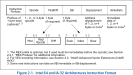
\includegraphics[scale=0.8]{img/intel_instruction_format.pdf}
    \end{center}
\end{frame}

\begin{frame}[fragile]{Formato de instrucción - ARM}
    \begin{center}
     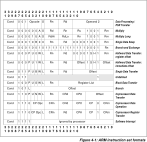
\includegraphics[scale=0.55]{img/arm_instruction_format.pdf}
    \end{center}
\end{frame}

\begin{frame}[fragile,t]{Modos de direccionamiento}
    Para ilustrar un conjunto de modos de direccionamiento vamos a utilizar la instrucción \texttt{MOV}.
    \begin{itemize}
    \item<1-> \small \textbf{Inmediato}\\
    \hspace{0.2cm} \textcolor{verdeuca}{\texttt{MOV R0, 0x1234}} \hspace{0.2cm} $\rightarrow$ \hspace{0.2cm} \textcolor{verdeuca}{\texttt{R0 = 0x1234}}\\
    \hspace{0.4cm} \scriptsize Mueve un valor inmediato codificado como parte de la instrucción a un registro.
    \item<2-> \small \textbf{Directo}\\
    \hspace{0.2cm} \textcolor{verdeuca}{\texttt{MOV R0, R1}} \hspace{0.2cm} $\rightarrow$ \hspace{0.2cm} \textcolor{verdeuca}{\texttt{R0 = R1}}\\
    \hspace{0.4cm} \scriptsize Mueve el valor de un registro a otro registro. 
    \item<3-> \small \textbf{Indirecto}\\
    \hspace{0.2cm} \textcolor{verdeuca}{\texttt{MOV R0, [0x1234]}} \hspace{0.2cm} $\rightarrow$ \hspace{0.2cm} \textcolor{verdeuca}{\texttt{R0 = MEM[0x1234]}}\\
    \hspace{0.4cm} \scriptsize Mueve el contenido de una dirección de memoria, codificada como parte de la instrucción, a un registro.
    \item<4-> \small \textbf{Indirecto a registro}\\
    \hspace{0.2cm} \textcolor{verdeuca}{\texttt{MOV R0, [R1]}} \hspace{0.2cm} $\rightarrow$ \hspace{0.2cm} \textcolor{verdeuca}{\texttt{R0 = MEM[R1]}}\\
    \hspace{0.4cm} \scriptsize Mueve el contenido de una dirección de memoria apuntada por un registro a otro registro.
    \item<5-> \small \textbf{Indexado}\\
    \hspace{0.2cm} \textcolor{verdeuca}{\texttt{MOV R0, [R1 + 0x20]}} \hspace{0.2cm} $\rightarrow$ \hspace{0.2cm} \textcolor{verdeuca}{\texttt{R0 = MEM[R1+0x20] }}\\
    \hspace{0.4cm} \scriptsize Mueve el contenido de una dirección de memoria apuntada por un registro más un desplazamiento a otro registro.
    \end{itemize}
\end{frame}

\begin{frame}[fragile]
    \frametitle{\texttt{big-endian} vs \texttt{little-endian}}
    La memoria generalmente almacena datos de a \textbf{byte} (8 bits).\\
    Se puede decir que funciona como un \emph{gran} \textbf{arreglo de bytes}.\\
    \bigskip
    Por ejemplo, el número 1810 como entero de 16 bits (2 bytes):\\
    \begin{center}
    \texttt{0000011100010010b} \hspace{0.2cm} $\rightarrow$ \hspace{0.2cm} \texttt{0000 0111 0001 0010 b} \hspace{0.2cm} $\rightarrow$ \hspace{0.2cm} \texttt{07 12 h}
    \end{center}
    \pause
    Tenemos que guardar dos bytes en memoria,
    \begin{itemize}
    \item \textcolor{naranjauca}{\texttt{big-endian}}\\
    El número se almacena comenzando por el \textbf{byte más significativo}:
    \begin{center} \renewcommand{\tabcolsep}{0pt}
    \begin{tabular}{C{3em}|C{3em}|C{3em}|C{3em}|C{3em}|C{3em}|C{3em}|C{3em}}
    \multicolumn{1}{>{\scriptsize}c}{25}& \multicolumn{1}{>{\scriptsize}c}{26}&
    \multicolumn{1}{>{\scriptsize}c}{27}& \multicolumn{1}{>{\scriptsize}c}{28}&
    \multicolumn{1}{>{\scriptsize}c}{29}& \multicolumn{1}{>{\scriptsize}c}{30}&
    \multicolumn{1}{>{\scriptsize}c}{31}& \multicolumn{1}{>{\scriptsize}c}{32}\\
    \hline
    & \cellcolor[gray]{0.95} & \cellcolor[gray]{0.95} & 
    \cellcolor[gray]{0.9} \texttt{07} & \cellcolor[gray]{0.9} \texttt{12} & 
    \cellcolor[gray]{0.95} & \cellcolor[gray]{0.95} &  \\
    \hline
    \end{tabular}
    \end{center}
    \item \textcolor{naranjauca}{\texttt{little-endian}}\\
    El número se almacena comenzando por el \textbf{byte menos significativo}:
    \begin{center} \renewcommand{\tabcolsep}{0pt}
    \begin{tabular}{C{3em}|C{3em}|C{3em}|C{3em}|C{3em}|C{3em}|C{3em}|C{3em}}
    \multicolumn{1}{>{\scriptsize}c}{25}& \multicolumn{1}{>{\scriptsize}c}{26}&
    \multicolumn{1}{>{\scriptsize}c}{27}& \multicolumn{1}{>{\scriptsize}c}{28}&
    \multicolumn{1}{>{\scriptsize}c}{29}& \multicolumn{1}{>{\scriptsize}c}{30}&
    \multicolumn{1}{>{\scriptsize}c}{31}& \multicolumn{1}{>{\scriptsize}c}{32}\\
    \hline
    & \cellcolor[gray]{0.95} & \cellcolor[gray]{0.95} & 
    \cellcolor[gray]{0.9} \texttt{12} & \cellcolor[gray]{0.9} \texttt{07} & 
    \cellcolor[gray]{0.95} & \cellcolor[gray]{0.95} &  \\
    \hline
    \end{tabular}
    \end{center}
    \end{itemize}
\end{frame}

% \begin{frame}[fragile,t]
% - Programa
% - Memoria de un programa
% - Codigo
% - Datos
% - - Pila
% - - Data solo lectura
% - - Data lectura escritura
% - - Heap (memoria dinamica)
% \end{frame}

\begin{frame}[fragile]
    \frametitle{Bibliografía}
    \begin{itemize}
     \setlength\itemsep{0.5cm}
    \item[-] \small Tanenbaum, “Organización de Computadoras. Un Enfoque Estructurado”, 4ta Edición, 2000.\\
    \begin{itemize}
%      \item \textbf{Capítulo 2 - Organización de los Sistemas de Computadora} - Páginas 39-45
     \item \textbf{Capítulo 5 - El nivel de Arquitectura del Conjunto de Instrucciones}\\
     \begin{itemize}
     \item 5.3 Formatos de Instrucciones - Páginas 322 - 332
     \item 5.4 Direccionamiento - Páginas 332 - 338
     \end{itemize}
    \end{itemize}
    \item[-] \small Null, “Essentials of Computer Organization and Architecture”, 5th Edition, 2018.\\
    \begin{itemize}
     \item Secciones:
     \begin{itemize}
    \item 1.9 The Von Neumann Model
    \item 1.10 Non-Von Neumann Models
%      \item 4.2 CPU Basics and Organization
%      \item 4.3 The Bus
%      \item 4.6 Memory Organization and Adressing
%      \item 4.8 MARIE
%      \item 4.9 Instruction Processing
     \item 4.14 Real-Word Examples of Computer Architectures
     \end{itemize}
    \end{itemize}
%     \item[-] \small Silberschatz, “Fundamentos de Sistemas Operativos”, 7ma Edición, 2006.\\
%     \item[-] \small Tanenbaum, “Modern Operating Systems”, 4th Edition, 2015.\\
    \end{itemize}
     \textcolor{naranjauca}{Referencias}
     \begin{itemize}
    \item[-] Especificación de la Arquitectura OrgaSmall\\ \small \url{https://github.com/fokerman/microOrgaSmall/}
    \end{itemize}
\end{frame}

% \begin{frame}[fragile]
%     \frametitle{Ejercicios}
%     Con lo visto, ya pueden resolver todos los ejercicios de la Guía de Lógica Digital.
% \end{frame}

\begin{frame}[plain]
    \begin{center}
    \vspace{2cm}
    \huge ¡Gracias!\\
    \vspace{2cm}
    \normalsize Recuerden leer los comentarios adjuntos\\ en cada clase por aclaraciones.
    \end{center}
\end{frame}


\begin{frame}[fragile,t]{Organización de OrgaSmall}
    La arquitectura \emph{OrgaSmall} está completamente implementada en Logisim.\\
    \begin{textblock}{100}(10,20)
    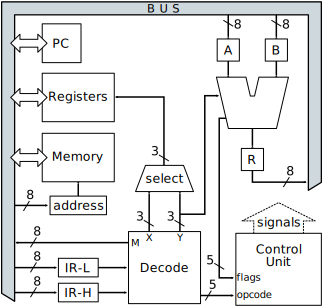
\includegraphics[scale=0.6]{img/arquitectura_micro.pdf}
    \end{textblock}
    \begin{textblock}{70}(70,20)
    Sus componentes son:\\
    \begin{itemize}
    \item \textbf{RB} - \texttt{Registers} (Banco de Registros)
    \item \textbf{PC} - \texttt{PC} (Contador de Programa)
    \item \textbf{ALU} - \texttt{ALU} (Unidad Aritmético Lógica)
    \item \textbf{MM} - \texttt{Memory} (Memoria)
    \item \textbf{DE} - \texttt{Decode} (Decodificador de Instrucciones)
    \item \textbf{CU} - \texttt{ControlUnit} (Unidad de Control)
    \end{itemize}
    Todos están conectados a un bus común, y sus señales comandadas por la Unidad de Control.
    \end{textblock}
\end{frame}

\begin{frame}[fragile,t]{Organización de OrgaSmall}
La unidad de control cuenta con las siguientes señales de entrada y salida:\\
\begin{center}
\small
\begin{tabular}{l|p{7cm}}
\textbf{Señales} & \textbf{Descripción} \\
\hline
\texttt{inOpcode(5)}                                                 & Entrada de \emph{Opcode}.\\
\texttt{flags(3)}                                                    & Entrada de \emph{flags}.\\
\hline
\texttt{RB\_enIn(1)} y \texttt{RB\_enOut(1)}                         & Señales de habilitación para Registros.\\
\texttt{RB\_inSelect(1)} y \texttt{RB\_outSelect(1)}                 & Señales de selección para Registros.\\
\hline
\texttt{MM\_enOut(1)} y \texttt{MM\_load(1)}                         & Señales para la Memoria.\\
\texttt{MM\_enAddr(1)}                                               & Habilita cargar la dirección.\\
\hline
\texttt{ALU\_enA(1)}, \texttt{ALU\_enB(1)} y \texttt{ALU\_enOut(1)}  & Señales de habilitación de la ALU.\\
\texttt{ALU\_opW(1)}, \texttt{ALU\_OP(4)}                            & Señales de control de la ALU.\\
\hline
\texttt{PC\_load(1)}, \texttt{PC\_inc(1)} y \texttt{PC\_enOut(1)}    & Señales de control de PC.\\
\hline
\texttt{DE\_enOutImm(1)}                                             & Habilita la entrada al bus de un valor inmediato.\\
\texttt{DE\_loadL(8)} y \texttt{DE\_loadH(8)}                        & Indica cargar la mitad alta o baja.\\
\hline
\end{tabular}
\end{center}
Cada instrucción de 16 bits se decodifica a una secuencia de estas señales.
\end{frame}

\begin{frame}[fragile,t]{Herramientas para OrgaSmall}
    \begin{textblock}{40}(10,35)
    Para simplificar el desarrollo se proveen dos programas en \texttt{python}:\\
    \end{textblock}
    \begin{textblock}{50}(60,10)
    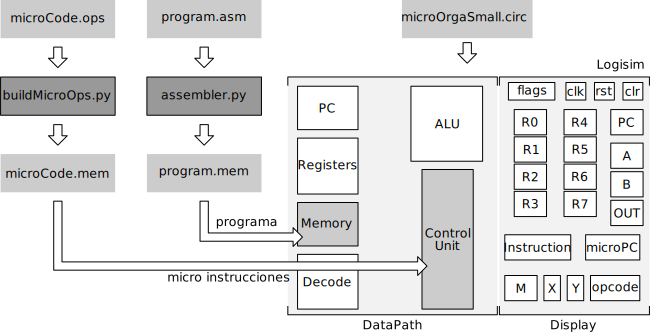
\includegraphics[scale=0.5]{img/herramientas.pdf}
    \end{textblock}
    \begin{textblock}{140}(10,55)
    \textcolor{naranjauca}{\texttt{assembler.py}}\\
    Toma un archivo en ensamblador de \emph{OrgaSmall} (\texttt{.asm}) y genera un archivo (\texttt{.mem}) para cargar en la memoria de la máquina en Logisim.\\
    \textcolor{naranjauca}{\texttt{buildMicroOps.py}}\\
    Toma un archivo con micro-operaciones para la máquina \emph{OrgaSmall} (\texttt{.ops}) y genera un archivo (\texttt{.mem}) para cargar en la memoria de micro-instrucciones de la máquina en Logisim.
    \end{textblock}
\end{frame}

\begin{frame}[fragile,t]{Micro-instrucciones de OrgaSmall}
\small
El programa \texttt{buildMicroOps.py} toma un archivo con señales de la siguiente forma:
\scriptsize
\begin{verbatim}
<binary_opcode>:
<signal_1> <signal_2> ... <signal_n>
...
<signal_1> <signal_2> ... <signal_n>
\end{verbatim}
\small
\texttt{binary\_opcode}: \textcolor{verdeuca}{Indica el Opcode de la instrucción a codificar.}\\
\texttt{signal\_x}: \textcolor{verdeuca}{Corresponde a una señal en 1 (o \texttt{signal\_x=val}).}\\
\bigskip
Ejemplo para la instrucción ADD:
\scriptsize
    \begin{verbatim}
00001: ; ADD
    RB_enOut  ALU_enA  RB_selectIndexOut=0   ; ALU_A := Rx
    RB_enOut  ALU_enB  RB_selectIndexOut=1   ; ALU_B := Ry
    ALU_OP=ADD ALU_opW                       ; ALU_ADD
    RB_enIn   ALU_enOut RB_selectIndexIn=0   ; Rx := ALU_OUT
    reset_microOp
\end{verbatim}
\small
Además se puede utilizar el carácter ``;'' para indicar comentarios.
\end{frame}

\begin{frame}[fragile,t]{Organización de OrgaSmall}
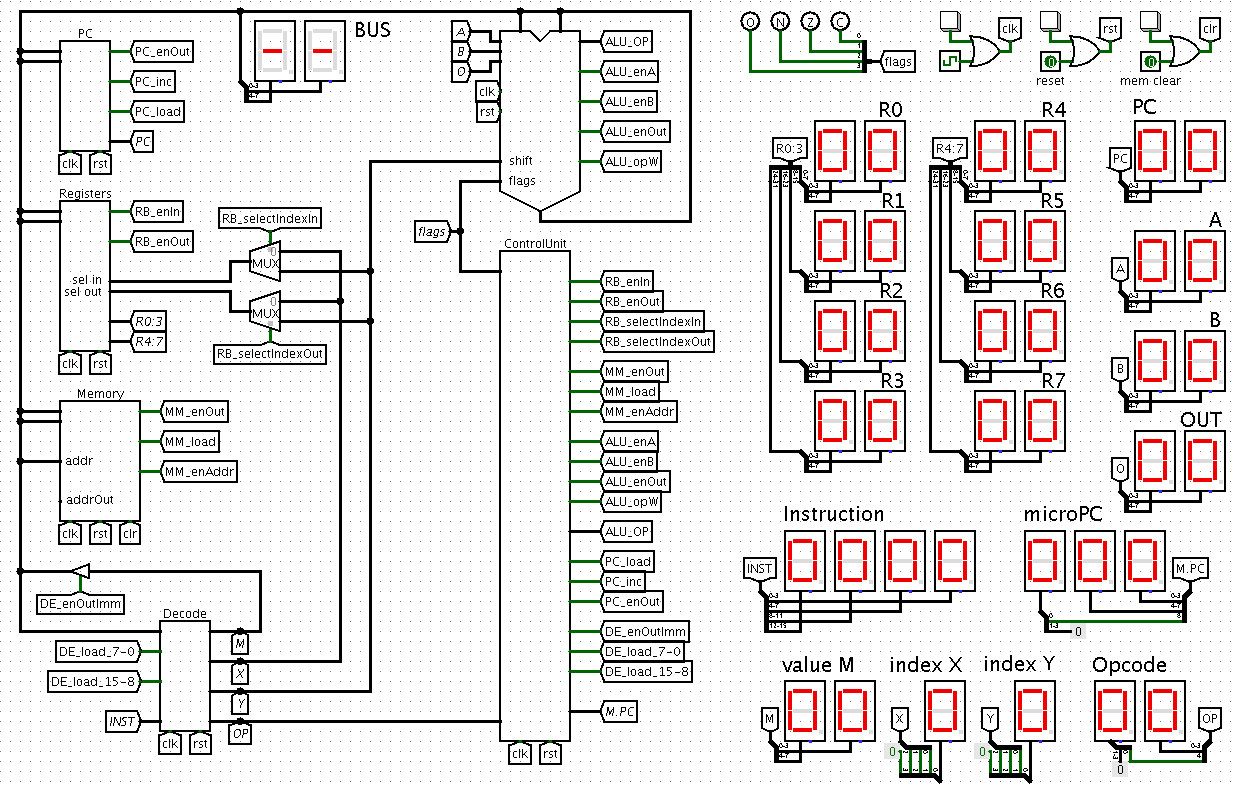
\includegraphics[scale=0.27]{img/0_dataPath.png}
\end{frame}

\begin{frame}[fragile,t]{Organización de OrgaSmall}{\textbf{RB} - \texttt{Registers} (Banco de Registros)}
    \begin{center} 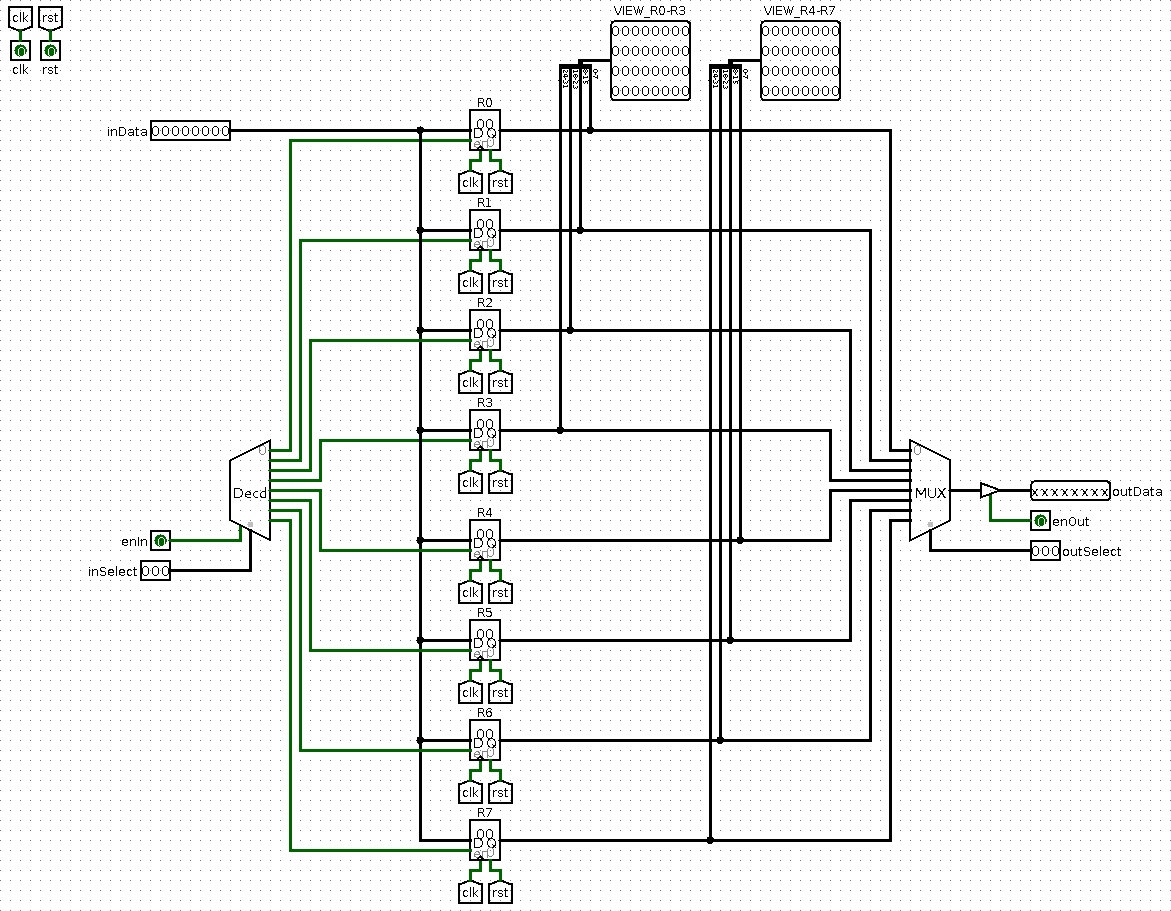
\includegraphics[scale=0.22]{img/1_registers.png} \end{center}
\end{frame}

\begin{frame}[fragile]{Organización de OrgaSmall}{\textbf{PC} - \texttt{PC} (Contador de Programa)}
    \begin{center} 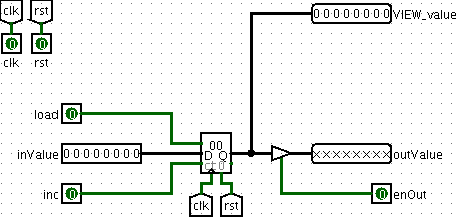
\includegraphics[scale=0.3]{img/2_PC.png} \end{center}
\end{frame}

\begin{frame}[fragile,t]{Organización de OrgaSmall}{\textbf{ALU} - \texttt{ALU} (Unidad Aritmético Lógica)}
    \begin{center} 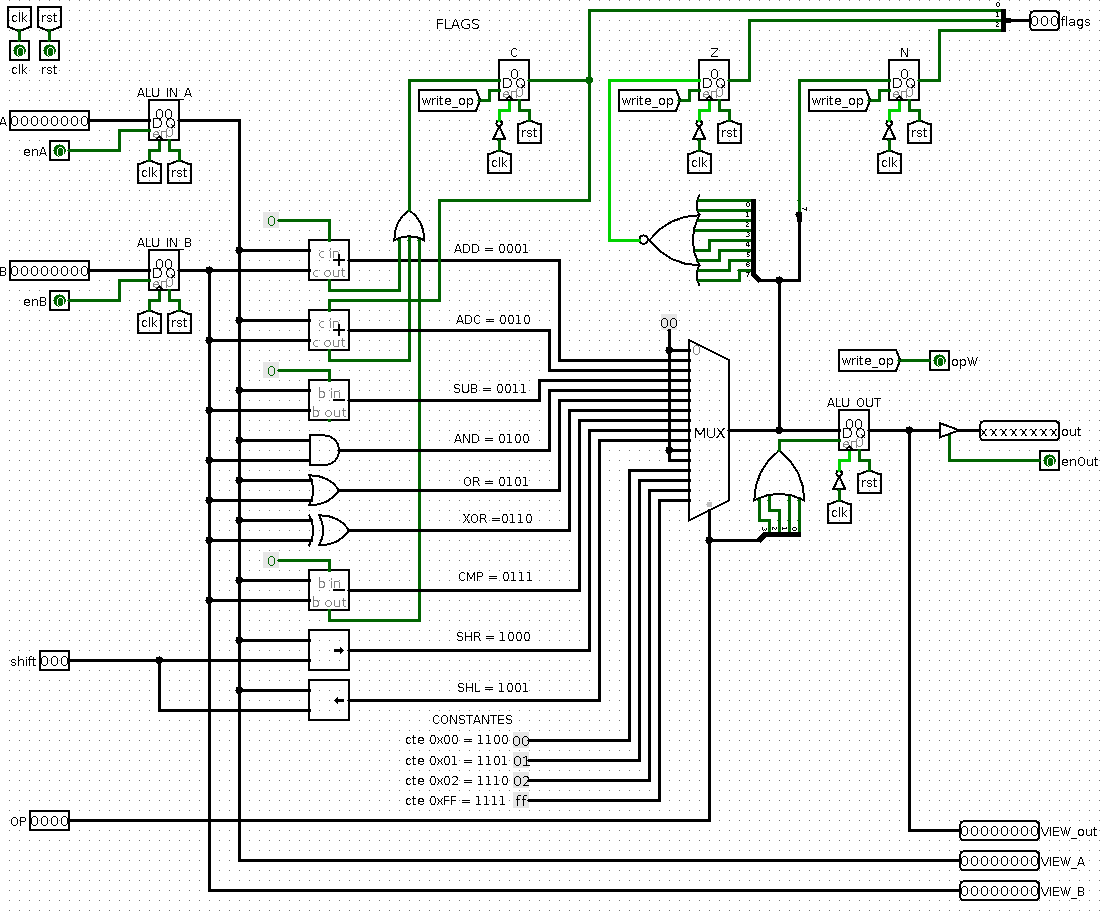
\includegraphics[scale=0.22]{img/4_ALU.png} \end{center}
\end{frame}

\begin{frame}[fragile,t]{Organización de OrgaSmall}{\textbf{MM} - \texttt{Memory} (Memoria)}
    \begin{center} 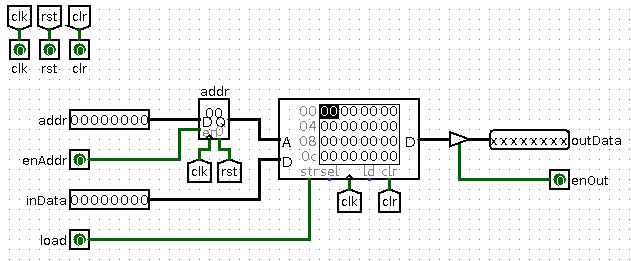
\includegraphics[scale=0.3]{img/5_Memory.png} \end{center}
\end{frame}

\begin{frame}[fragile,t]{Organización de OrgaSmall}{\textbf{DE} - \texttt{Decode} (Decodificador de Instrucciones)}
    \begin{center} 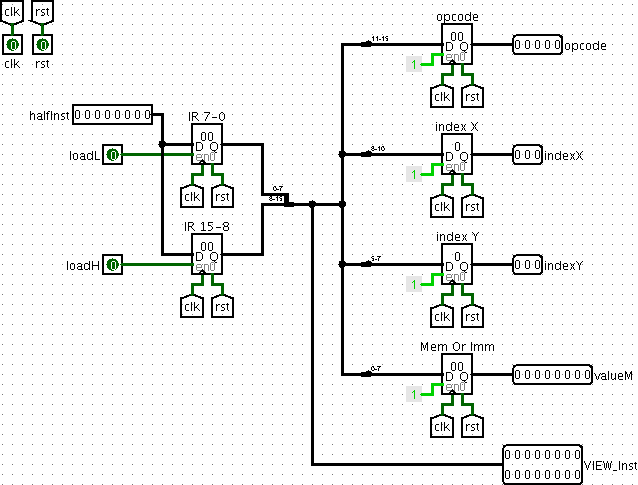
\includegraphics[scale=0.3]{img/6_Decode.png} \end{center}
\end{frame}

\begin{frame}[fragile,t]{Organización de OrgaSmall}{\textbf{CU} - \texttt{ControlUnit} (Unidad de Control)}
    \begin{center} 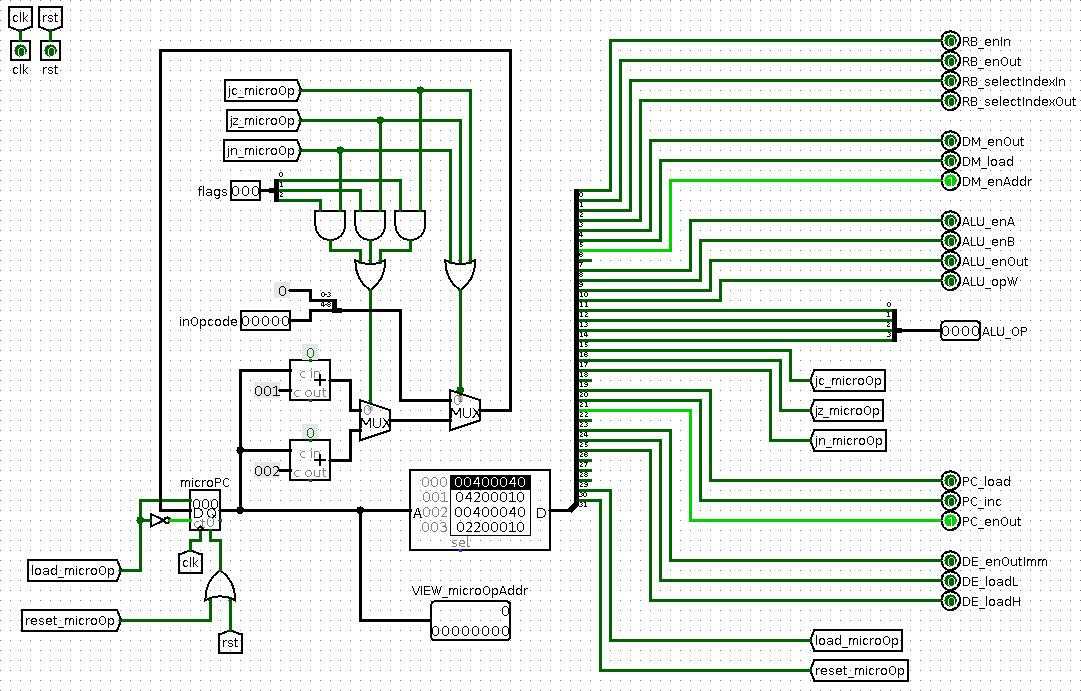
\includegraphics[scale=0.27]{img/7_ControlUnit.png} \end{center}
\end{frame}

\end{document}

% % % % % % % % % % % % % % % % % % 
% EJEMPLOS:

\begin{frame}[fragile]
    \frametitle{Bla}
    \begin{itemize}
    \item[-] Bla bla \textbf{ble} bla bla
    \item[-] Bla bla \textbf{ble} bla bla
    \end{itemize}
\end{frame}

\begin{frame}[fragile]
    \frametitle{Bla}
    \begin{block}{\texttt{BLA}}
    Bla Bla
    \end{block}
    \begin{multicols}{2}
    \begin{tabular}{ll}
    la & la \\
    \end{tabular}
    \columnbreak
    \begin{tabular}{ll}
    la & la \\
    \end{tabular}
    \end{multicols}
\end{frame}

\begin{frame}
    \frametitle{Bla}
    \begin{itemize}
    \item Bla bla
    \begin{center}
    \includegraphics[scale=0.7]{img/struct_aling.pdf}
    \end{center}
    Bla bla
    \end{itemize}
\end{frame}

\begin{frame}[fragile]
    \frametitle{Bla}
    \begin{textblock}{100}(10,10)
    Bla
    \end{textblock}
\end{frame}

\end{document}

